\documentclass{article}
\usepackage{amsmath, amssymb}
\usepackage{tikz}
\setlength{\parindent}{0pt}

\begin{document}

\textbf{MATH 1564 --- Notes 09/03}

\bigskip

A function $f$ is a device with input $x$ and output $f(x)$.

\medskip

One function is $f: \mathbb{R}^n \to \mathbb{R}^m$ ($\mathbb{R}^n$ is the \textbf{domain}, $\mathbb{R}^m$ is the \textbf{codomain}).

\medskip

\textbf{Example:} What's the domain and codomain of $x^2$? Domain $\in \mathbb{R}$, codomain $\in \mathbb{R}$.

\bigskip

\textbf{Definition:} The image (the range) of $f$ is the set $\{f(x) : x \text{ is in the domain}\}$.

\medskip

\textbf{Example:} The image of $f(x) = x^2$ is $f(x) \geq 0$.

\medskip

\textbf{Example:} Domain, codomain, and image of $f(x) = \frac{1}{x}$?
\[
\text{Domain} = \mathbb{R} - \{0\}, \qquad \text{Codomain} = \mathbb{R}, \qquad \text{Image} = \mathbb{R} - \{0\}.
\]

\bigskip

\textbf{Example:} Let $A$ be an $m \times n$ matrix. Define a function $T: \mathbb{R}^n \to \mathbb{R}^m$ given by $T(x) = Ax$.
\[
\text{Domain of } T = \mathbb{R}^n, \qquad \text{Codomain of } T = \mathbb{R}^m.
\]

\bigskip

\textbf{Theorem 1:} If $A = [a_1 \; \cdots \; a_n]$, then the image of $T$ is $\mathrm{span}\{a_1, a_2, \ldots, a_n\}$.

\newpage

\textbf{Proof:} Since $a_i$ = column $i$ of $A$,
\[
T(x) = [a_1 \; \cdots \; a_n] \begin{bmatrix} x_1 \\ \vdots \\ x_n \end{bmatrix} = x_1 a_1 + \cdots + x_n a_n.
\]
Since any $x$ is allowed, this covers all linear combinations of $a_1, \ldots, a_n$.

\bigskip

\textbf{Example:} Let $A$ be the zero matrix. Then $T(x) = Ax = 0$ for all $x$.

\bigskip

\textbf{Example:} $T: \mathbb{R}^n \to \mathbb{R}^n$ and $A = \begin{bmatrix} 1 & & 0 \\ & \ddots & \\ 0 & & 1 \end{bmatrix}$, the $n \times n$ identity matrix.
\[
T(x) = \begin{bmatrix} 1 & & 0 \\ & \ddots & \\ 0 & & 1 \end{bmatrix} \begin{bmatrix} x_1 \\ \vdots \\ x_n \end{bmatrix}
= x_1 \begin{bmatrix} 1 \\ 0 \\ \vdots \\ 0 \end{bmatrix} + x_2 \begin{bmatrix} 0 \\ 1 \\ \vdots \\ 0 \end{bmatrix} + \cdots + x_n \begin{bmatrix} 0 \\ \vdots \\ 0 \\ 1 \end{bmatrix} = x.
\]

\bigskip

\textbf{Example:} $T: \mathbb{R}^n \to \mathbb{R}^n$ and $A = \begin{bmatrix} c & & 0 \\ & \ddots & \\ 0 & & c \end{bmatrix}$ for some scalar $c$. Then $T(x) = cx$.

\newpage

\textbf{Example:} Projection of $\mathbb{R}^2$ onto the $x_1$-axis:
\[
T\left( \begin{bmatrix} x_1 \\ x_2 \end{bmatrix} \right) = \begin{bmatrix} 1 & 0 \\ 0 & 0 \end{bmatrix} \begin{bmatrix} x_1 \\ x_2 \end{bmatrix} = \begin{bmatrix} x_1 \\ 0 \end{bmatrix}.
\]

\bigskip

\textbf{Example:} Projection of $\mathbb{R}^2$ onto the $x_2$-axis:
\[
T\left( \begin{bmatrix} x_1 \\ x_2 \end{bmatrix} \right) = \begin{bmatrix} 0 & 0 \\ 0 & 1 \end{bmatrix} \begin{bmatrix} x_1 \\ x_2 \end{bmatrix} = \begin{bmatrix} 0 \\ x_2 \end{bmatrix}.
\]

\bigskip

\textbf{Reflection across the $x_1$-axis.}

\medskip

\textbf{Example:} $A = \begin{bmatrix} 1 & 0 \\ 0 & -1 \end{bmatrix}$,
\[
T\left( \begin{bmatrix} x_1 \\ x_2 \end{bmatrix} \right) = \begin{bmatrix} 1 & 0 \\ 0 & -1 \end{bmatrix} \begin{bmatrix} x_1 \\ x_2 \end{bmatrix} = \begin{bmatrix} x_1 \\ -x_2 \end{bmatrix}.
\]

\begin{center}
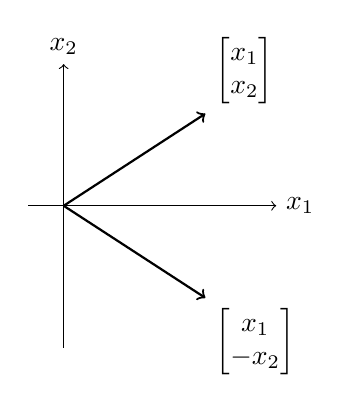
\begin{tikzpicture}[scale=0.9]
\draw[->] (-0.5,0) -- (3,0) node[right] {$x_1$};
\draw[->] (0,-2) -- (0,2) node[above] {$x_2$};
\draw[->,thick] (0,0) -- (2,1.3) node[above right] {$\begin{bmatrix} x_1 \\ x_2 \end{bmatrix}$};
\draw[->,thick] (0,0) -- (2,-1.3) node[below right] {$\begin{bmatrix} x_1 \\ -x_2 \end{bmatrix}$};
\end{tikzpicture}
\end{center}

\bigskip

\textbf{Reflection across $\{x_1 = x_2\}$.}

\medskip

\textbf{Example:} $A = \begin{bmatrix} 0 & 1 \\ 1 & 0 \end{bmatrix}$,
\[
T\left( \begin{bmatrix} x_1 \\ x_2 \end{bmatrix} \right) = \begin{bmatrix} 0 & 1 \\ 1 & 0 \end{bmatrix} \begin{bmatrix} x_1 \\ x_2 \end{bmatrix} = \begin{bmatrix} x_2 \\ x_1 \end{bmatrix}.
\]

\begin{center}
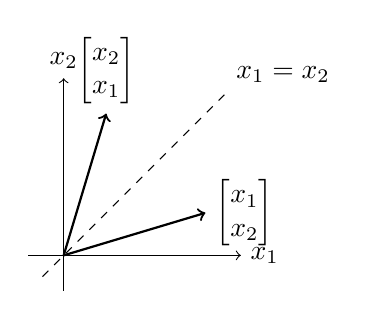
\begin{tikzpicture}[scale=0.9]
\draw[->] (-0.5,0) -- (2.5,0) node[right] {$x_1$};
\draw[->] (0,-0.5) -- (0,2.5) node[above] {$x_2$};
\draw[dashed] (-0.3,-0.3) -- (2.3,2.3) node[above right] {$x_1 = x_2$};
\draw[->,thick] (0,0) -- (2,0.6) node[right] {$\begin{bmatrix} x_1 \\ x_2 \end{bmatrix}$};
\draw[->,thick] (0,0) -- (0.6,2) node[above] {$\begin{bmatrix} x_2 \\ x_1 \end{bmatrix}$};
\end{tikzpicture}
\end{center}

\newpage

\textbf{Definition:} A function (map, or transformation $T: \mathbb{R}^n \to \mathbb{R}^m$) is \textbf{linear} if:
\begin{enumerate}
\item[a)] $T(x+y) = T(x) + T(y) \quad \forall x, y \in \mathbb{R}^n$
\item[b)] $T(cx) = cT(x) \quad \forall c \in \mathbb{R}$
\end{enumerate}

\medskip

\textbf{Example (proof):} $T(x) = Ax$ is linear.
\[
T(x+y) = A(x+y) = [a_1 \; \cdots \; a_n] \begin{bmatrix} x_1+y_1 \\ \vdots \\ x_n+y_n \end{bmatrix}
= (x_1+y_1)a_1 + \cdots + (x_n+y_n)a_n
\]
\[
= x_1 a_1 + \cdots + x_n a_n + y_1 a_1 + \cdots + y_n a_n = Ax + Ay = T(x) + T(y).
\]
Similarly, $T(cx) = A(cx) = cAx = cT(x)$.

\newpage

\textbf{Theorem 2:} Let $T: \mathbb{R}^n \to \mathbb{R}^m$ be a map. Then $T$ is linear $\iff$
\[
T(c_1 v_1 + \cdots + c_k v_k) = c_1 T(v_1) + \cdots + c_k T(v_k)
\]
for all vectors $v_i$ and scalars $c_i$, $i \in [1,k]$.

\medskip

\textbf{Proof:} Take $k=2$ and $c_1 = 1 = c_2$, and $k=1$ (these are exactly properties (a) and (b) of linearity). Induct on $k$:
\begin{align*}
T(c_1 v_1 + \cdots + c_k v_k) &= T(c_1 v_1 + \cdots + c_{k-1} v_{k-1}) + T(c_k v_k) \\
&= c_1 T(v_1) + \cdots + c_{k-1} T(v_{k-1}) + c_k T(v_k).
\end{align*}

\medskip

$T$ is linear iff $T$ takes linear combinations to linear combinations.

\bigskip

\textbf{Example:} Suppose $T(v_1) = 0 = T(v_2)$. Then $T$ takes $\mathrm{span}\{v_1, v_2\}$ to
\[
T(c_1 v_1 + c_2 v_2) = c_1 T(v_1) + c_2 T(v_2) = 0 + 0 = 0.
\]

\newpage

\textbf{Theorem 3:} Any linear map takes the zero vector to the zero vector.

\medskip

\textbf{Proof:} Since $0 + y = y$,
\[
T(0+y) = T(0) + T(y) \quad \Rightarrow \quad T(y) = T(0) + T(y) \quad \Rightarrow \quad T(0) = 0.
\]

\bigskip

\textbf{Example:} Let $T(x) = Ax$ where $A = \begin{bmatrix} 1 & 1 \\ 0 & 1 \\ 1 & 1 \end{bmatrix}$ and $b = \begin{bmatrix} 7 \\ 5 \\ 7 \end{bmatrix}$.
\[
\text{Domain of } T \text{ is } \mathbb{R}^2 \; (2 \text{ columns}), \qquad \text{Codomain of } T \text{ is } \mathbb{R}^3 \; (3 \text{ rows}).
\]

\medskip

Is $b$ in the image of $T$? Solve $Ax = T(x) = b$:
\[
\left[ \begin{array}{cc|c} 1 & 1 & 7 \\ 0 & 1 & 5 \\ 1 & 1 & 7 \end{array} \right]
\to
\left[ \begin{array}{cc|c} 1 & 1 & 7 \\ 0 & 1 & 5 \\ 0 & 0 & 0 \end{array} \right]
\to
\left[ \begin{array}{cc|c} 1 & 0 & 2 \\ 0 & 1 & 5 \\ 0 & 0 & 0 \end{array} \right]
\]
Yes, we have a consistent solution: $x = \begin{bmatrix} 2 \\ 5 \end{bmatrix}$.

\newpage

\textbf{Definition:} The standard basis vectors $e_1, \ldots, e_n$ in $\mathbb{R}^n$ are the columns of the identity $n \times n$ matrix
\[
I_n = \begin{bmatrix} 1 & & 0 \\ & \ddots & \\ 0 & & 1 \end{bmatrix}, \qquad \text{namely } e_i = \text{column } i \text{ of } I_n.
\]

\medskip

\textbf{Property:}
\[
\begin{bmatrix} x_1 \\ \vdots \\ x_n \end{bmatrix} = x_1 e_1 + \cdots + x_n e_n = I_n \begin{bmatrix} x_1 \\ \vdots \\ x_n \end{bmatrix}.
\]

\bigskip

If $A = [v_1 \; \cdots \; v_n]$ is an $m \times n$ matrix and $v_i$ = column $i$ of $A$, then
\[
Ae_i = v_i, \qquad T(x) = Ax, \qquad T(e_i) = v_i.
\]
\[
[v_1 \; \cdots \; v_n] \begin{bmatrix} 1 \\ 0 \\ \vdots \\ 0 \end{bmatrix} = 1 \cdot v_1 + 0 \cdot v_2 + \cdots + 0 \cdot v_n = v_1.
\]

\newpage

\textbf{Theorem 4 (Standard matrix of a linear map):} If $T: \mathbb{R}^n \to \mathbb{R}^m$ is a linear map and $A = [T(e_1) \; \cdots \; T(e_n)]$ is the $m \times n$ matrix whose $i$th column is $T(e_i)$, then
\[
T(x) = Ax, \quad \forall x.
\]

\medskip

\textbf{Proof:}
\begin{align*}
T(x) &= T(x_1 e_1 + \cdots + x_n e_n) \\
&\overset{\text{linear}}{=} x_1 T(e_1) + \cdots + x_n T(e_n) \\
&= [T(e_1) \; \cdots \; T(e_n)] \begin{bmatrix} x_1 \\ \vdots \\ x_n \end{bmatrix} = Ax.
\end{align*}

\bigskip

A linear map $\mathbb{R}^n \to \mathbb{R}^m$ is another description of an $m \times n$ matrix.

\medskip

\textbf{How to check if a map $\mathbb{R}^n \to \mathbb{R}^m$ is linear:} Check if $T(x) = Ax$ for some $A$.

\medskip

\textbf{Example:} Is $T\left( \begin{bmatrix} x_1 \\ x_2 \end{bmatrix} \right) = \begin{bmatrix} x_1 + x_2 \\ x_2 + 1 \end{bmatrix}$ linear?
\[
[T(e_1) \; T(e_2)] \begin{bmatrix} x_1 \\ x_2 \end{bmatrix} = \begin{bmatrix} 1 & 1 \\ 1 & 2 \end{bmatrix} \begin{bmatrix} x_1 \\ x_2 \end{bmatrix} = \begin{bmatrix} x_1 + x_2 \\ x_1 + 2x_2 \end{bmatrix} \neq \begin{bmatrix} x_1 + x_2 \\ x_2 + 1 \end{bmatrix}.
\]
Indeed $T(0) = \begin{bmatrix} 0 \\ 1 \end{bmatrix} \neq 0$, so by Theorem 3, $T$ is not linear.

\newpage

\textbf{Example:} Let $T: \mathbb{R}^2 \to \mathbb{R}^2$ rotate counterclockwise by angle $\varphi \in \left(0, \frac{\pi}{2}\right)$.

\begin{center}
\begin{tikzpicture}[scale=1.3]
\draw[->] (-1.5,0) -- (1.5,0);
\draw[->] (0,-1.5) -- (0,1.5);
\draw[->,thick] (0,0) -- (1.2,0.5) node[right] {$x$};
\draw[->,thick] (0,0) -- (0.7,1.15) node[above] {$T(x)$};
\draw (0.5,0) arc (0:43:0.5);
\node at (0.65,0.28) {$\varphi$};
\end{tikzpicture}
\end{center}

\medskip

What's the standard matrix of $T$? Since $e_1 = \begin{bmatrix} 1 \\ 0 \end{bmatrix}$ rotates to angle $\varphi$ and $e_2 = \begin{bmatrix} 0 \\ 1 \end{bmatrix}$ rotates to angle $\varphi + \frac{\pi}{2}$:
\[
T(e_1) = \begin{bmatrix} \cos\varphi \\ \sin\varphi \end{bmatrix}, \qquad T(e_2) = \begin{bmatrix} -\sin\varphi \\ \cos\varphi \end{bmatrix}.
\]

\begin{center}
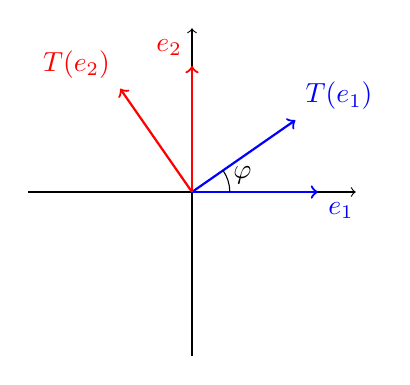
\begin{tikzpicture}[scale=1.6]
\draw[->] (-1.3,0) -- (1.3,0);
\draw[->] (0,-1.3) -- (0,1.3);
\draw[->,thick,blue] (0,0) -- (1,0) node[below right] {$e_1$};
\draw[->,thick,blue] (0,0) -- (0.82,0.57) node[above right] {$T(e_1)$};
\draw[->,thick,red] (0,0) -- (0,1) node[above left] {$e_2$};
\draw[->,thick,red] (0,0) -- (-0.57,0.82) node[above left] {$T(e_2)$};
\draw (0.3,0) arc (0:35:0.3);
\node at (0.4,0.13) {$\varphi$};
\end{tikzpicture}
\end{center}

\medskip

So the standard matrix is
\[
[T(e_1) \; T(e_2)] = \begin{bmatrix} \cos\varphi & -\sin\varphi \\ \sin\varphi & \cos\varphi \end{bmatrix}.
\]
One can show that this matrix works for any $\varphi$ (not just $\varphi \in (0, \pi/2)$).

\newpage

\textbf{Definition:} A function $f$ is \textbf{onto} if the image of $f$ equals the codomain of $f$. Thus $T: \mathbb{R}^n \to \mathbb{R}^m$ is onto if for every $b$ in $\mathbb{R}^m$ there is $x$ in $\mathbb{R}^n$ with $T(x) = b$.

\bigskip

\textbf{Theorem 5:} If $T(x) = Ax$, then $T$ is onto $\iff$ each row of $A$ is pivotal.

\medskip

\textbf{Proof:} $Ax$ is consistent for every $b$ $\iff$ each row of $A$ is pivotal.

\medskip

(Remark: for a square matrix, invertible $\iff$ onto.)

\bigskip

\textbf{Definition:} A function $f$ is \textbf{one-to-one} if $u \neq v \Rightarrow f(u) \neq f(v)$ for any $u, v$ in the domain of $f$.

\medskip

\textbf{Example:} If $f(x) = x^2$, $f: \mathbb{R} \to \mathbb{R}$, is $f$ one-to-one? No.

\newpage

\textbf{Theorem 6:} Let $T(x) = Ax$ where $A$ is an $m \times n$ matrix. Then the following are equivalent:
\begin{enumerate}
\item $T$ is one-to-one.
\item $Ax = b$ has at most one solution.
\item $Ax = 0$ only has the zero solution.
\item Each column of $A$ is pivotal.
\end{enumerate}

\medskip

\textbf{Proof:} $2 \iff 3 \iff 4$ (given previously). $1 \iff 2$: since $T(x) = Ax$, (1) means that $T(x) = b$ has at most one solution, which is exactly what one-to-one means.

\bigskip

\textbf{Example:} Let $T\left( \begin{bmatrix} x_1 \\ x_2 \end{bmatrix} \right) = \begin{bmatrix} 3x_1 + x_2 \\ 5x_1 + 7x_2 \\ x_1 + 3x_2 \end{bmatrix}$.
\[
\text{Domain of } T = \mathbb{R}^2, \qquad \text{Codomain of } T = \mathbb{R}^3.
\]

\medskip

Is $T$ linear? If so, find its standard matrix.
\[
[T(e_1) \; T(e_2)] \begin{bmatrix} x_1 \\ x_2 \end{bmatrix} = \begin{bmatrix} 3 & 1 \\ 5 & 7 \\ 1 & 3 \end{bmatrix} \begin{bmatrix} x_1 \\ x_2 \end{bmatrix} = \begin{bmatrix} 3x_1+x_2 \\ 5x_1+7x_2 \\ x_1+3x_2 \end{bmatrix}
\]
$\therefore$ $T$ is linear, with standard matrix $\begin{bmatrix} 3 & 1 \\ 5 & 7 \\ 1 & 3 \end{bmatrix}$.

\medskip

Is $T$ one-to-one? Onto?
\[
\begin{bmatrix} 3 & 1 \\ 5 & 7 \\ 1 & 3 \end{bmatrix} \to \begin{bmatrix} 1 & 3 \\ 5 & 7 \\ 3 & 1 \end{bmatrix} \to \begin{bmatrix} 1 & 3 \\ 0 & -8 \\ 0 & -8 \end{bmatrix} \to \begin{bmatrix} 1 & 0 \\ 0 & 1 \\ 0 & 0 \end{bmatrix} \; (\text{RREF})
\]
Both columns are pivotal, so $T$ is one-to-one. Only 2 of the 3 rows are pivotal (row 3 is zero), so $T$ is \textbf{not} onto.

\end{document}
